% !TEX root = thesis.tex

\section{Results}\label{sec:results}
\subsection{Pupil size}
\begin{figure}[tp]
  \centering
  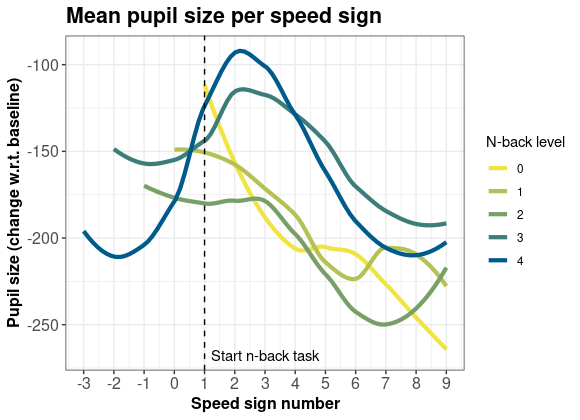
\includegraphics[width=7.5cm]{images/speed_sign_nback.png}
  \caption{Mean pupil size over the period between the appearance of two speed signs; bars represent standard error.
  The dashed vertical line indicates the moment that participants need to start performing the \(n\)-back task by regulating their speed according to the speed signs.
  Pupil size was corrected using subtractive baseline correction and is shown in arbitrary units. 
  The data were smoothed using the loess method.}
  \label{fig:ps-speed-sign}
\end{figure}

Figure~\ref{fig:ps-speed-sign} shows how the pupil size of participants changed within a trial.
There is a visible distinction between pupil size for low \(n\)-back levels (\(n = 0,1,2\)) and high \(n\)-back levels (\(n = 3,4\)).
Whereas high \(n\)-back levels show a peak in pupil size, low \(n\)-back levels show a decline from the start of the task.
Interestingly, compared to \(n = 3\) the peak for \(n = 4\) is higher but shows a sharper decline afterwards.
An explanation for this could be that participants focus their attention on the task at first but then quickly abandon the task because of its difficulty.
[This is confirmed by the increase in task error for the higher \(n\)-back levels as shown in Figure~.]

\begin{figure}[tp]
  \centering
  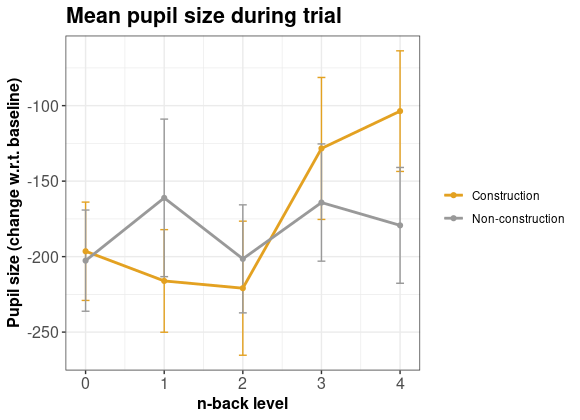
\includegraphics[width=7.5cm]{images/pupil_size_interaction.png}
  \caption{Mean pupil size during trial; bars represent standard error.
  Pupil size was corrected using subtractive baseline correction and is shown in arbitrary units.}
  \label{fig:mean-ps}
\end{figure}


\subsection{Fixations on speedometer}

\begin{figure}[tp]
  \centering
  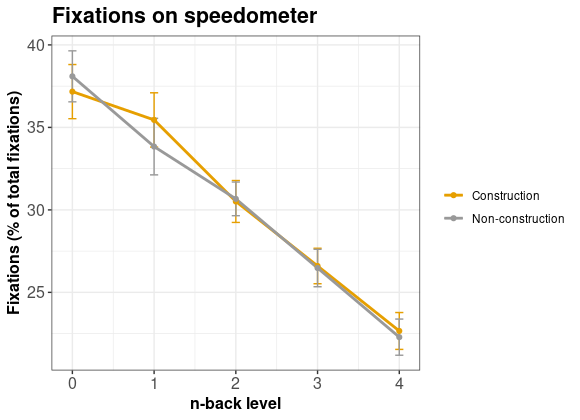
\includegraphics[width=7.5cm]{images/speedometer_interaction.png}
  \caption{Number of fixations on the speedometer as a percentage of the total number of fixations for that trial.}
  \label{fig:fix-speedometer}
\end{figure}